\section{Manipulate Conductivity in Quantum Hall System}

Now using the relations derived in Eq. \eqref{5.34} and Eq. \eqref{7.17} we can derive that
\begin{equation} \label{8.1}
  \Gamma_n = \qty(\frac{\hbar }{2\tau(\varepsilon_n)}) =
  \frac{1}{2}\Gamma^{00}_{N}(\tilde{I})
\end{equation}
and this will be
\begin{equation} \label{8.2}
  \Gamma_n(\tilde{I}) = 0.12\times
  \qty[
  \frac
  {\int_{-\infty}^{\infty} d {k}_1 \;
  J_0^2\qty(2.090\sqrt{\tilde{I}}\times{k}_1)
  \qty|
  \int_{-\infty}^{\infty} d{k}_2 \;
  \tilde{\chi}_{N}\qty(2.342 \times k_2)
  \tilde{\chi}_{N}\qty(2.342 \times \qty[{k}_1 - {k}_2])|^2}
  {\int_{-\infty}^{\infty} d {k}_1 \;
  \qty|
  \int_{-\infty}^{\infty} d{k}_2 \;
  \tilde{\chi}_{0}\qty(2.342 \times k_2)
  \tilde{\chi}_{0}\qty(2.342 \times \qty[{k}_1 - {k}_2])|^2}
  ]^{1/2} \text{meV}
\end{equation}

\noindent
In addition we can calculate the cyclotron energy as
\begin{equation} \label{8.3}
  \hbar\omega_0 = 1.95663 \;\text{meV}
\end{equation}
and
\begin{equation} \label{8.4}
  \gamma_n = \frac{\Gamma_n}{\hbar \omega_0} = 0.06133 \times \Lambda_n(\tilde{I}) \approx 0.061 \Lambda_n(\tilde{I})
\end{equation}

\noindent
Now we can use this into our conductivity expression derived in Eq. \eqref{7.23} and present the normalized transverse conductivity as a function of fermi energy and intensity of the dressing field
\begin{equation} \label{8.5}
  \begin{aligned}
    \sigma^{xx}(X_F,\tilde{I}) & =
    \sum_{n}
    \frac{\qty(n+1)}{0.0037\Lambda_n \Lambda_{n+1}}
    \qty[
      \frac{1}
      {
        1 + \qty(\frac{X_F - n -1}{0.06\Lambda_n})^2
      }
    ]
    \qty[
      \frac{1}
      {
        1 + \qty(\frac{X_F - n}{0.06\Lambda_{n+1}})^2
      }
    ]
  \end{aligned}
\end{equation}
where
\begin{equation} \label{8.6}
    \Lambda_n  =
    \qty[
    \frac
    {\int_{-\infty}^{\infty} d {k}_1 \;
    J_0^2\qty(2.090\sqrt{\tilde{I}}\times{k}_1)
    \qty|
    \int_{-\infty}^{\infty} d{k}_2 \;
    \tilde{\chi}_{n}\qty(2.342 \times k_2)
    \tilde{\chi}_{n}\qty(2.342 \times \qty[{k}_1 - {k}_2])|^2}
    {\int_{-\infty}^{\infty} d {k}_1 \;
    \qty|
    \int_{-\infty}^{\infty} d{k}_2 \;
    \tilde{\chi}_{0}\qty(2.342 \times k_2)
    \tilde{\chi}_{0}\qty(2.342 \times \qty[{k}_1 - {k}_2])|^2}
    ]^{1/2}.
\end{equation}
\hfill$\blacksquare$

\noindent
Now using Eq. \eqref{8.6} we can calculate the normalized broadening of each Landau levels as given in Table \ref{tab:8.1}.

\begin{table}[ht!]
\begin{center}
\begin{tabular}{ |c|c|c|c|c|c|c|c|c|c|c|c| }
 \hline
 ${\tilde{I}}$
 & $n=0$ & $n=1$ & $n=2$ & $n=3$ & $n=4$ & $n=5$ & $n=6$ & $n=7$ & $n=8$ & $n=9$
 & $n=10$
 \\ [0.5ex] \hline\hline
 0  & $1.0000$ & $0.8660$ & $0.8004$ & $0.7578$ & $0.7266$
 & $0.7021$ & $0.6821$ & $0.6653$ & $0.6507$ & $0.6380$& $0.6267$ \\ \hline
 1  & $0.8546$ & $0.7037$ & $0.6502$ & $0.6114$ & $0.5810$
 & $0.5584$ & $0.5416$ & $0.5280$ & $0.5160$ & $0.5050$ & $0.4948$ \\ \hline
 4  & $0.6875$ & $0.6345$ & $0.5902$ & $0.5528$ & $0.5307$
 & $0.5118$ & $0.4958$ & $0.4840$ & $0.4730$ & $0.4629$  & $0.4547$ \\ \hline
 9  & $0.5936$ & $0.5539$ & $0.5333$ & $0.5180$ & $0.5006$
 & $0.4812$ & $0.4685$ & $0.4564$ & $0.4469$ & $0.4377$  & $0.4305$ \\ \hline
\end{tabular}
\caption {\label{tab:8.1} $\Lambda_n$ values for each Landau level by changing  applied dressing field intensity ($\tilde{I}$). }
\end{center}
\end{table}

\noindent
Using above values we can analyse the changes can be done to the transverse conductivity using apllied dressing field. As given in Figure \ref{fig:8.1} and \ref{fig:8.2} we can manipulate the conductivity using external dressing field. When the applied field's intensity increase the broadening of energy bands of Landau levels get reduced the conductivity also get decrease all the regions except the peak point of the energy band. Using this manipulation we can filter the conductivity which is change with the Fermi level. Since Fermi level can be change with the applied gate voltage of the material this can be used as a 2D switch for optoelectonic applications. Using the applied dressing field we can fine tune the switching mechanism.

\begin{figure}[ht!]
  \centering
  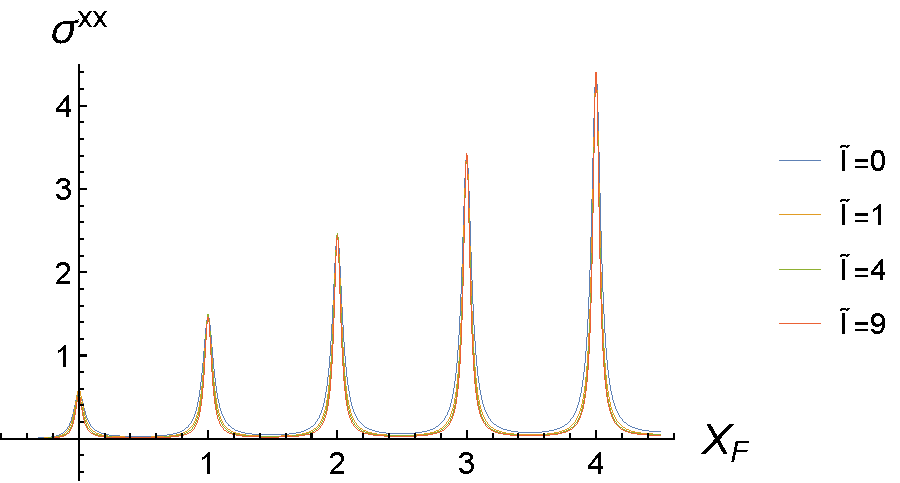
\includegraphics[scale=1]{figures/fig81.pdf}
  \caption{Normalized transverse conductivity against Fermi level ($X_F$) with different intensities ($\tilde{I}$) of dressing field.}
  \label{fig:8.1}
\end{figure}
\begin{figure}[ht!]
  \centering
  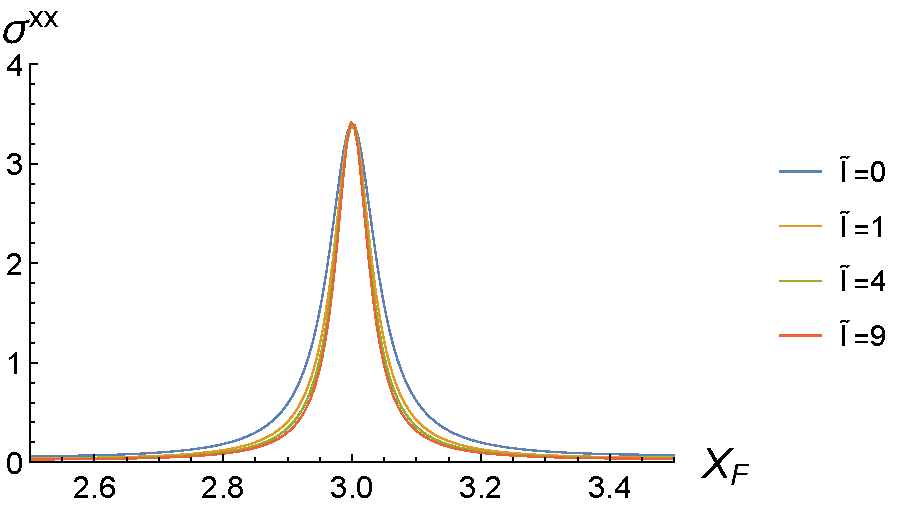
\includegraphics[scale=1]{figures/fig82.pdf}
  \caption{$3$rd Landau level's normalized transverse conductivity against Fermi level ($X_F$) with different intensities ($\tilde{I}$) of dressing field.}
  \label{fig:8.2}
\end{figure}
